\documentclass{beamer}

\usepackage[utf8]{inputenc}
\usepackage[T1]{fontenc}
\usepackage{amsmath}
\usepackage{amsfonts}
\usepackage{amssymb}
\usepackage{amssymb, bm}
\usepackage{mathtools, bm}
\usepackage{mathrsfs}
\usepackage{stmaryrd}
\usepackage{graphicx}
\usepackage{tikz}
%\usepackage[]{algorithm2e}
\usepackage[]{algorithm}
\usepackage[]{algorithmic}
\usepackage{framed}
% fonction pour définir une fonction 
\newcommand{\fonction}[5]{
    \begin{array}{ccccc}
#1 & : & #2 & \to & #3\\
    & & #4 & \mapsto & #5\\ 
    \end{array}
}
\setbeamerfont{section in toc}{size=\small}
\setbeamerfont{subsection in toc}{size=\small}
\begin{document}
\title{
    {\normalsize\textbf{Résolution de Formules Booléennes Quantifiées\\à l'aide de Réseaux de Neurones}}\\
	{\large Université Paris-Diderot}
}
\author{
	{Mohammed Younes Megrini}\\
	{Nicolas Nalpon}
}
\date{10 juin 2016}

\frame{\titlepage}

\frame{
	\frametitle{Introduction : AlphaGo} 
	\includegraphics[scale=.3]{alphago.jpg}
}

\frame{
	\frametitle{Introduction : Deep-Q Learning Atari}
	\begin{center}
	\includegraphics[scale=.5]{atari-75.png}
	\end{center}
}

\frame{\frametitle{Table des matières}\tableofcontents[subsubsectionstyle=hide]} 

\section{Réseaux de neurones}
\frame{\frametitle{Table des matières}\tableofcontents[currentsection, subsubsectionstyle=show/hide/show]} 

\subsection{Modèle de McCulloh-Pitts}
\frame{\frametitle{Modèle de McCulloh-Pitts}
\begin{center}
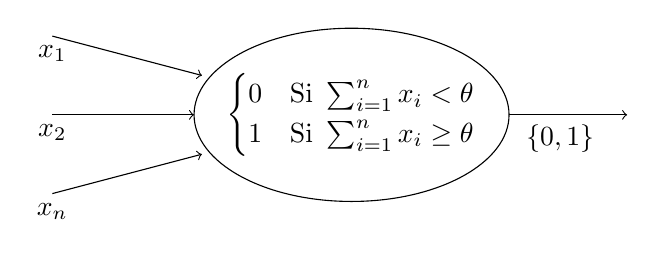
\begin{tikzpicture}[]
	%\draw[help lines, thick] (0,0) grid (9,5);
	\draw[->] (0.7,2.5) node [below] {$x_{2}$}-- (2.5,2.5);
	\draw[->] (6.5,2.5)-- node[below, align=center] {$\left\{0,1\right\}$} (7.8,2.5)-- (8,2.5);
	\draw[->] (0.7,3.5) node [below] {$x_{1}$} -- (2.6,3);
	\draw[->] (0.7,1.5) node [below] {$x_{n}$}-- (2.6,2);
	\draw (4.5,2.5) node {$ \begin{cases} 0 &\mbox{Si } \sum_{i=1}^{n} {x_i} < \theta \\ 1 & \mbox{Si } \sum_{i=1}^{n} {x_i} \geq \theta \end{cases} $} circle [x radius= 2, y radius=1.1];
\end{tikzpicture}
\end{center}
}

\subsubsection{Neurone Perceptron}
\frame{\frametitle{Neurone Perceptron}
\begin{center}
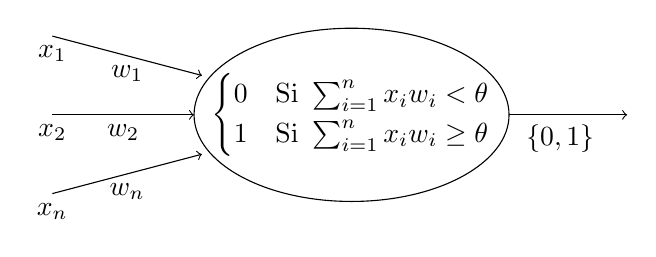
\begin{tikzpicture}[]
	%\draw[help lines, thick] (0,0) grid (9,5);
	\draw[->] (0.7,2.5) node [below] {$x_{2}$}-- node [below] {$w_{2}$} (2.5,2.5);
	\draw[->] (6.5,2.5)-- node[below, align=center] {$\left\{0,1\right\}$} (7.8,2.5)-- (8,2.5);
	\draw[->] (0.7,3.5) node [below] {$x_{1}$} -- node [below] {$w_{1}$} (2.6,3);
	\draw[->] (0.7,1.5) node [below] {$x_{n}$}-- node [below] {$w_{n}$} (2.6,2);
	\draw (4.5,2.5) node {$ \begin{cases} 0 &\mbox{Si } \sum_{i=1}^{n} {x_iw_i} < \theta \\ 1 & \mbox{Si } \sum_{i=1}^{n} {x_iw_i} \geq \theta \end{cases} $} circle [x radius= 2, y radius=1.1];
\end{tikzpicture}
\end{center}
}

\subsubsection{Neurone Sigmoïde}
\frame{\frametitle{Neurone Sigmoïde}
\begin{center}
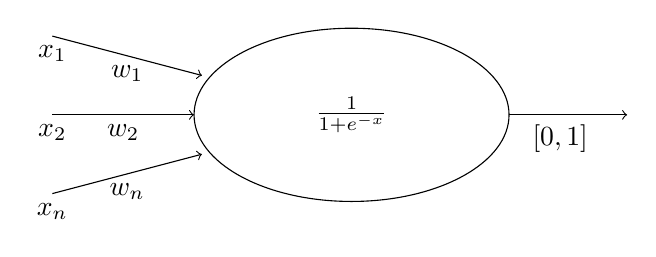
\begin{tikzpicture}[]
	%\draw[help lines, thick] (0,0) grid (9,5);
	\draw[->] (0.7,2.5) node [below] {$x_{2}$}-- node [below] {$w_{2}$} (2.5,2.5);
	\draw[->] (6.5,2.5)-- node[below, align=center] {$\left[0,1\right]$} (7.8,2.5)-- (8,2.5);
	\draw[->] (0.7,3.5) node [below] {$x_{1}$} -- node [below] {$w_{1}$} (2.6,3);
	\draw[->] (0.7,1.5) node [below] {$x_{n}$}-- node [below] {$w_{n}$} (2.6,2);
	\draw (4.5,2.5) node {$ \frac{1}{1+e^{-x}}  $} circle [x radius= 2, y radius=1.1];
\end{tikzpicture}
\end{center}
}

\subsection{Réseau de Neurones}
\frame{\frametitle{Réseau de Neurones}
\def\layersep{2.5cm}
\begin{center}
\begin{tikzpicture}[shorten >=1pt,->,draw=black!50, node distance=\layersep]
    \tikzstyle{every pin edge}=[<-,shorten <=1pt]
    \tikzstyle{neuron}=[circle,fill=black!25,minimum size=17pt,inner sep=0pt]
    \tikzstyle{input neuron}=[neuron, fill=black!20];
    \tikzstyle{output neuron}=[neuron, fill=black!30];
    \tikzstyle{hidden neuron}=[neuron, fill=black!80];
    \tikzstyle{annot} = [text width=4em, text centered]

    % Draw the input layer nodes
    \foreach \name / \y in {1,...,4}
    % This is the same as writing \foreach \name / \y in {1/1,2/2,3/3,4/4}
        \node[input neuron, pin=left:Entrée \y] (I-\name) at (0,-\y) {};

    % Draw the hidden layer nodes
    \foreach \name / \y in {1,...,5}
        \path[yshift=0.5cm]
            node[hidden neuron] (H-\name) at (\layersep,-\y cm) {};

    % Draw the output layer node
    \node[output neuron,pin={[pin edge={->}]right:Sortie}, right of=H-3] (O) {};

    % Connect every node in the input layer with every node in the
    % hidden layer.
    \foreach \source in {1,...,4}
        \foreach \dest in {1,...,5}
            \path (I-\source) edge (H-\dest);

    % Connect every node in the hidden layer with the output layer
    \foreach \source in {1,...,5}
        \path (H-\source) edge (O);

    % Annotate the layers
    \node[annot,above of=H-1, node distance=1cm] (hl) {Couche cachée};
    \node[annot,left of=hl] {Couche d'entrée};
    \node[annot,right of=hl] {Couche de sortie};
\end{tikzpicture}
\end{center}
}

\section{Apprentissage profond}
\frame{\frametitle{Table des matières}\tableofcontents[currentsection, subsubsectionstyle=show/hide/show]} 

\subsection{Fonction d'erreur quadratique moyenne}
\frame{\frametitle{Fonction d'erreur quadratique moyenne}
\begin{center}
\[\fonction{C_{x}}{\mathbb{R}^{n+1}}{\mathbb{R}}{(w_1,.....,w_{n+1})}{\frac{1}{2}(y(x)-\Phi_{x}(w_1,.....,w_{n+1}))^{2}}\]
\end{center}
}

\subsection{Descente de Gradient}
\frame{\frametitle{Descente de Gradient}
\begin{algorithm}[H]
	\caption{Descente de Gradient}
	\begin{algorithmic}[1]
	\REQUIRE $x_{0} \in \mathbb{R}^{n+1}$, $c\in \mathbb{N}$, $\varepsilon \ge 0$
	\STATE$k=0$
	\WHILE{$\mid \mid \nabla f(x_{k}) \mid \mid  \ge \varepsilon$ and $k \neq c  $}
		\STATE Calcul de $\nabla f(x_{k})$ \; % calcule avec un e ou sans e 
		\STATE Calcul de $\alpha_{k} > 0 $ \;
		\STATE $ x_{k+1} = x_{k} - \alpha_{k} \nabla f(x_{k}) $ \;
		\STATE k++; 
	\ENDWHILE
	\end{algorithmic}
\end{algorithm}
}
\frame{\frametitle{Descente de Gradient}
\begin{algorithm}[H]
	\caption{Calcul du pas d'apprentissage}
	\begin{algorithmic}[1]
	\REQUIRE $x_{0}$ vecteur poids qu'on choisit initialement \\ 
	$k=0$
	\STATE Calculer $\nabla f(x_{K})$ \; 
	\STATE Choisir $\alpha_{k}$ afin de minimiser la fonction $h(\alpha) = f(x_{k}-\alpha \nabla f(x_{k}))$;
	\end{algorithmic}
\end{algorithm}
}

\subsection{Rétropropagation}
\frame{\frametitle{Table des matières}\tableofcontents[currentsubsection, subsubsectionstyle=show/show/hide]} 
\frame{\frametitle{Rétro-propagation}
\begin{center}
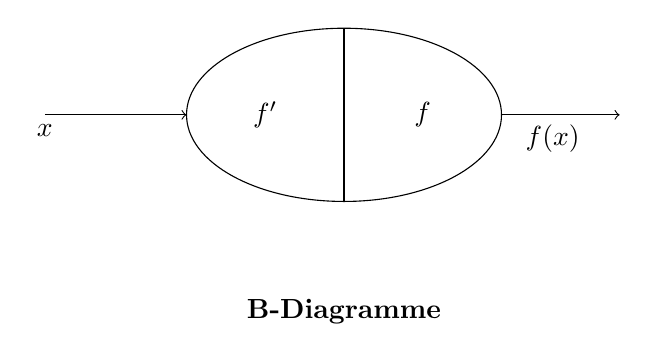
\begin{tikzpicture}[]
	%\draw[help lines, thick] (0,0) grid (9,5);
	\draw[->] (0.7,2.5) node [below] {$x$}-- (2.5,2.5);
	\draw[->] (6.5,2.5)-- node[below, align=center] {$f(x)$} (7.8,2.5)--(8,2.5);
	\draw (4.5,1.4)--(4.5,3.6);	
	\draw (4.5,2.5) circle [x radius= 2, y radius=1.1];
	\draw (3.5,2.5) node { $f'$ };
	\draw (5.5,2.5) node { $f$ };
	\draw (4.5,0) node { \textbf{B-Diagramme} };
\end{tikzpicture}
\end{center}
}
\subsubsection{Rétropropagation : feed-forward}
\frame{\frametitle{Rétro-propagation : \textit{feed-forward}}
\begin{center}
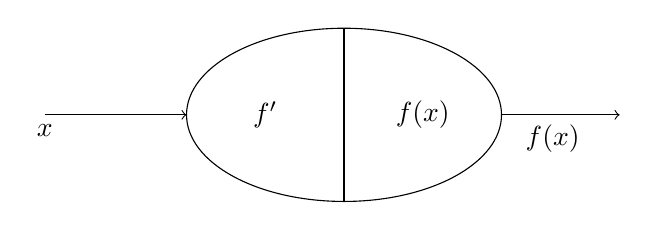
\begin{tikzpicture}[]
	%\draw[help lines, thick] (0,0) grid (9,5);
	\draw[->] (0.7,2.5) node [below] {$x$}-- (2.5,2.5);
	\draw[->] (6.5,2.5)-- node[below, align=center] {$f(x)$} (7.8,2.5)--(8,2.5);
	\draw (4.5,1.4)--(4.5,3.6);	
	\draw (4.5,2.5) circle [x radius= 2, y radius=1.1];
	\draw (3.5,2.5) node { $f'$ };
	\draw (5.5,2.5) node { $f(x)$ };
\end{tikzpicture}
\end{center}
}
\subsubsection{Rétropropagation : backpropagation}
\frame{\frametitle{Rétropropagation : \textit{backpropagation}}
\begin{center}
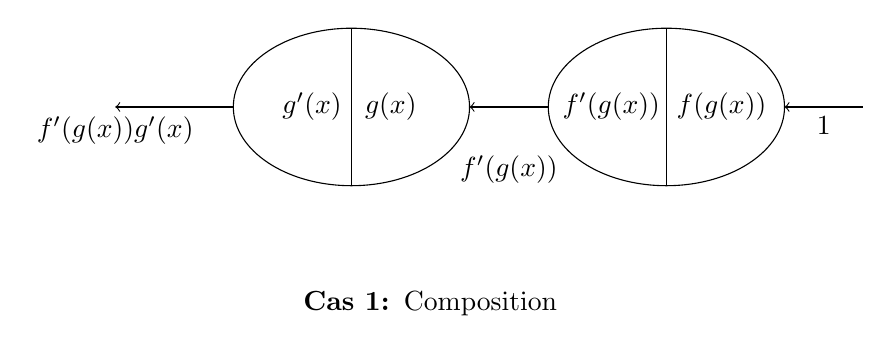
\begin{tikzpicture}[]
	%\draw[help lines, thick] (-1,0) grid (9,5);
	\draw[<-] (-2,2.5) node [below] {$f'(g(x))g'(x)$} -- (-0.5,2.5);
	\draw[<-] (6.5,2.5)-- node [below] {$1$}(7.5,2.5);
	\draw[<-] (2.5,2.5) --(3.5,2.5);
	\draw (3,2) node [below] {$f'(g(x))$};
	\draw (1,3.5)--(1,1.5);
	\draw (5,3.5)--(5,1.5);
	\draw (1,2.5) circle [x radius= 1.5, y radius=1];
	\draw (5,2.5) circle [x radius= 1.5, y radius=1];
	\draw (0.5,2.5) node {$g'(x)$};
	\draw (1.5,2.5) node {$g(x)$};
	\draw (4.3,2.5) node {$f'(g(x))$};
	\draw (5.7,2.5) node {$f(g(x))$};
	\draw (2,0) node { \textbf{Cas 1: }Composition };
\end{tikzpicture}
\end{center}
}
\frame{\frametitle{Rétropropagation : \textit{backpropagation}}
\begin{center}
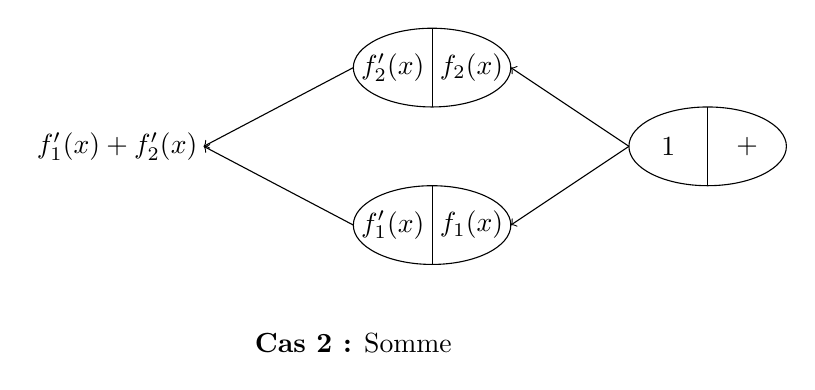
\begin{tikzpicture}[]
	%\draw[help lines, thick] (0,0) grid (9,5);
	\draw [<-] (4,1.5)--(5.5,2.5);
	\draw [<-] (4,3.5)--(5.5,2.5);
	\draw [->] (2,1.5)--(0.1,2.5);
	\draw [->] (2,3.5)--(0.1,2.5);
	\draw  (3,1)--(3,2);
	\draw  (3,3)--(3,4);
	\draw  (6.5,3)--(6.5,2);
	\draw (-1,2.5) node {$f'_{1}(x)+f'_2(x)$};
	\draw (2.5,1.5) node {$f'_{1}(x)$};
	\draw (2.5,3.5) node {$f'_2(x)$};
	\draw (3.5,1.5) node {$f_{1}(x)$};
	\draw (3.5,3.5) node {$f_2(x)$};
	\draw (7,2.5) node {$+$};
	\draw (6,2.5) node {$1$};
	\draw (3,1.5) circle [x radius= 1, y radius=0.5];
	\draw (3,3.5) circle [x radius= 1, y radius=0.5];
	\draw (6.5,2.5) circle [x radius= 1, y radius=0.5];
	\draw (2,0) node { \textbf{Cas 2 :} Somme};
\end{tikzpicture}
\end{center}
}
\frame{\frametitle{Rétropropagation : \textit{backpropagation}}
\begin{center}
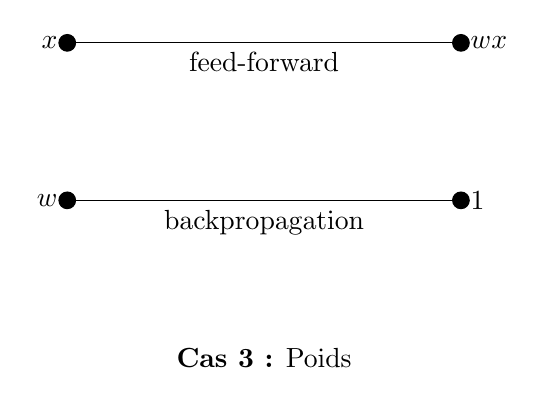
\begin{tikzpicture}[]
	%\draw[help lines, thick] (0,0) grid (9,5);
	\filldraw (2,2)[fill=black] circle (3pt);
	\draw (2,2)[left] node {$w$};
	\filldraw (7,2) [fill=black] circle (3pt);
	\draw (7,2)[right] node {$1$};
	\draw (2,2)--(7,2);
	\filldraw (2,4) [fill=black] circle (3pt);
	\draw (2,4)[left] node {$x$};
	\filldraw (7,4) [fill=black] circle (3pt);
	\draw (7,4)[right] node {$wx$};
	\draw (4.5,2) node [below] {backpropagation};
	\draw (4.5,4) node [below] {feed-forward};
	\draw (2,4)--(7,4);
	\draw (4.5,0) node { \textbf{Cas 3 :} Poids};
\end{tikzpicture}
\end{center}
}

\section{QBF-SAT}
\frame{\frametitle{Table des matières}\tableofcontents[currentsection, subsubsectionstyle=show/hide/show]} 

\subsection{Modèle des deux joueurs}
\frame{\frametitle{Modèle des deux joueurs}
\begin{center}
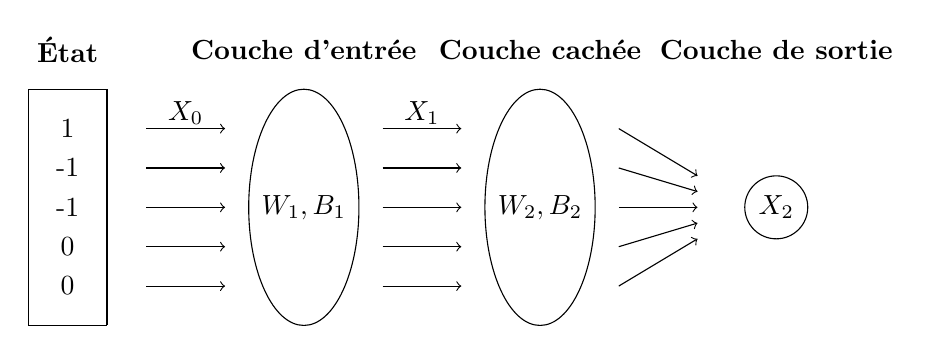
\begin{tikzpicture}[]
	%\draw[help lines, thick] (0,0) grid (11,5);
	\draw (3.5,2.5) node {$W_1,B_1$} circle [x radius=.7, y radius=1.5];
	\draw (6.5,2.5) node {$W_2,B_2$} circle [x radius=.7, y radius=1.5];
	\draw (9.5,2.5) node {$X_2$} circle [x radius=0.4, y radius=0.4];
	\draw [->] (1.5,1.5)--(2.5,1.5);
	\draw [->] (1.5,2)--(2.5,2);
	\draw [->] (1.5,2.5)--(2.5,2.5);
	\draw [->] (1.5,3)--(2.5,3);
	\draw [->] (1.5,3.5)--(2.5,3.5);
	\draw [->] (4.5,1.5)--(5.5,1.5);
	\draw [->] (4.5,2)--(5.5,2);
	\draw [->] (4.5,2.5)--(5.5,2.5);
	\draw [->] (4.5,3)--(5.5,3);
	\draw [->] (4.5,3.5)--(5.5,3.5);
	\draw [->] (7.5,1.5)--(8.5,2.1);
	\draw [->] (7.5,2)--(8.5,2.3);
	\draw [->] (7.5,2.5)--(8.5,2.5);
	\draw [->] (7.5,3)--(8.5,2.7);
	\draw [->] (7.5,3.5)--(8.5,2.9);
	\draw (0,4)--(1,4);
	\draw (0,4)--(0,1); 
	\draw (1,4)--(1,1); 
	\draw (0,1)--(1,1);
	\draw (0.5,3.5) node{1};
	\draw (0.5,3) node{-1};
	\draw (0.5,2.5) node{-1};
	\draw (0.5,2) node{0};
	\draw (0.5,1.5) node{0};
	\draw (.5,4.5) node {\textbf{État}}; 
	\draw (2,3.7) node {\textbf{$X_0$}}; 
	\draw (5,3.7) node {\textbf{$X_1$}};
	\draw (3.5,4.5) node {\textbf{Couche d'entrée}}; 
	\draw (6.5,4.5) node {\textbf{Couche cachée}}; 
	\draw (9.5,4.5) node {\textbf{Couche de sortie}}; 
\end{tikzpicture}
\end{center}
\[ X_{i+1} = S(W_{i+1}X_i+B_{i+1}) \]
}
\subsection{Pré-requis}
\frame{\frametitle{Table des matières}\tableofcontents[currentsubsection, subsubsectionstyle=show/show/hide]}
\subsubsection{Librairie Torch}
\frame{\frametitle{Librairie Torch}
\begin{center}	
	\includegraphics[scale=.7]{torch.jpg}
\end{center}
}
\frame{\frametitle{Librairie Torch}
	\includegraphics[scale=.3]{torch.jpg}	
	\begin{framed}
		function init()\\
		\quad local net = nn.Sequential()\\
    \quad net:add(nn.Linear(variables, variables))\\
    \quad net:add(nn.Sigmoid())\\
    \quad net:add(nn.Linear(variables, output))\\
    \quad net:add(nn.Sigmoid())\\
    \quad return net\\
   end
	
	\end{framed}
}

\subsubsection{Format QDimacs}
\frame{\frametitle{Format QDimacs}
Formule booléenne quantifiée normale conjonctive :
\[\exists x_5 \forall x_1 \forall x_4 \exists x_3 \forall x_2 \quad (x_1 \land \neg x_2 \land x_4 ) \lor (\neg x_3 \land x_4 \land x_5)\]
\pause
Format QDimacs :
\begin{framed}
\texttt{\\
p cnf 5 2\\ 
	a 1 4 0\\
	e 3 0\\
	a 2 0\\
	1 -2 4 0\\
	-3 4 5 0
}
\end{framed}
}
\subsection{Algorithme d'apprentissage de QBF-SAT}
\frame{\frametitle{Algorithme d'apprentissage de QBF-SAT}
\begin{algorithm}[H]
	\caption{Deep QBF-SAT Learning}
	\begin{algorithmic}[1]
	\REQUIRE  $k$ 
	\WHILE{$ cmp < k$}
	\STATE  s, r = result(session())
	\STATE  us, uv, es, ev = build(s, r);
	\STATE store(us, uv, es, ev);
	\STATE train(uni, uniMset, uniMval);
	\STATE train(exi, exiMset, exiMval);
	\STATE percentage(r)
	\STATE $cmp++$;
	\ENDWHILE
	\end{algorithmic}
	\end{algorithm}
}

\frame{\frametitle{Conclusion}
\begin{center}	
	\includegraphics[scale=.4]{terminal.jpg}
\end{center}
}
\end{document}

